\documentclass[uplatex]{jsarticle}
\usepackage[utf8]{inputenc}

\usepackage{amsmath}
\usepackage[dvipdfmx]{graphicx}
\usepackage{resume}  % resume用スタイル
\usepackage{udline}  % 下線用
\usepackage{comment} % 複数行コメント
\pagestyle{plain}
 
\begin{document}
\twocolumn[
    \beginheader{令和5年度 コンピュータサイエンス学部 中間発表}{2023}{8}{9}{井上 研究室}
    \title{VR環境時の落下感覚に姿勢の角度変化が与える影響の調査}
    \author{C0B20205 武田 夢音 (Yumene Takeda)}
    \endheader
]
\vspace{3mm}

%%ページ番号
\setcounter{page}{9}

\section{はじめに}
近年,VR機器の高性能化・低廉化による普及に伴い,VRを利用した研究やサービスが増加した.

落下感覚についての研究も盛んに行われ,VRバンジージャンプといった
VRと落下を組み合わせたイベントも登場した.

今までに行われた落下感覚についての研究により,姿勢と落下感覚が関係していることが判明しており,それらから姿勢は伏臥位をとった状態が比較的落下感覚が強くなることが分かっている.

しかし,姿勢に関する研究は立位や座位,伏臥位などの大まかな姿勢をとった状態で不動で落下した場合を検証したのみであり,体の角度や動きといった細かな部分までは研究されていない.

そこで,本研究では伏臥位の状態のまま体の角度を変化させられるデバイスを開発し,それを用いて伏臥位をとった状態での体の角度と落下角度の関係,そして落下中に角度を変化させた場合の落下感覚の変化についての調査を目的とする.


\section{関連研究}
東山らの研究\cite{vection}はロールベクション(刺激によって反対方向に回転していると錯覚する効果)に姿勢が与える影響についての分析を行っており,被験者に5種類の体勢を取らせて視覚刺激を与えることで発生するベクションの強度や発生速度についての実験を行っている.結果から,ベクションの知覚が最も早くなるのはうつ伏せと仰向けであり,ベクションが筋肉系の活動状態(姿勢の制御)による影響を受けることが示された.

奥川らの研究\cite{spatial_stimulation_effect_falling}はVR空間における視覚刺激と体勢によって発生する落下感覚の分析を行っており,落下時に見える風景の空間周波数と落下時の体勢を数パターン用意し,それぞれの落下感覚を比較する実験を行った.結果から,空間周波数は高いほど落下感覚が高まり体勢は伏臥位が最も落下感覚が高まるという結果が得られた.


 \begin{figure}[tb]
  % width や height で絶対的な大きさ指定をすることもできる
  \centering
  \fbox{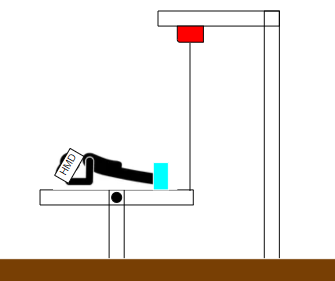
\includegraphics[width=1\linewidth]{fig/main_system.png}}
  \caption{システム概要図}
  \label{fig:about_system}

  \centering
  \fbox{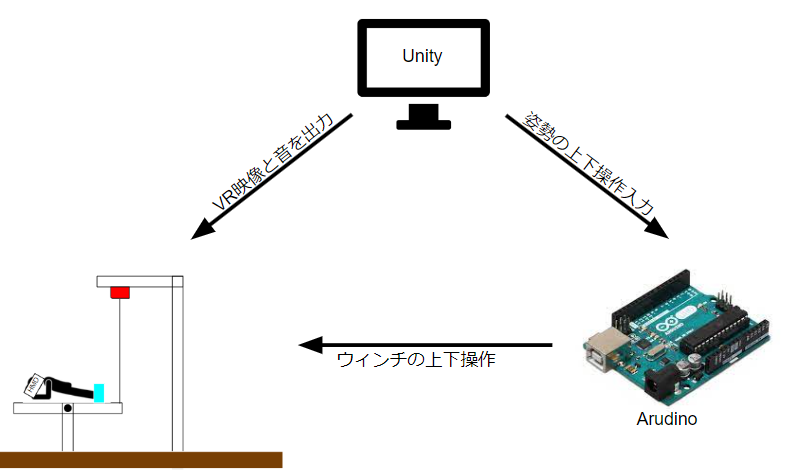
\includegraphics[width=1\linewidth]{fig/システム実装.png}}
  \caption{システム実装図}
  \label{fig:build_system}

\end{figure}

\section{伏臥位角度変更システム}
\subsection{システム概要}
システム概要の図を\figref{fig:about_system}に示す.プレイヤーは頭部にヘッドマウントディスプレイ(以降,HMD)を装着し,中央部で回転するように設置された台の上で伏臥位をとる.台の足側はウィンチにつながれており,VRシミュレーション中に体の角度を変えることができる.

足の周辺には固定具を設置し,頭が下になるような体制になっても台上で伏臥位をとれるよう固定する.

仮想空間にはビルの上などの高い場所にいるシチュエーションを用意し,被験者に対して数百メートルの高さから落下する映像を提示できるようにする.

また,ウィンチの上下操作はコンピュータで制御することで再現性のある実験を可能にする.

伏臥位になったプレイヤーはVR空間内で落下を体験し,落下に合わせて上下するウィンチによって体の角度が変化する.

\subsection{システム構成}
本研究ではシステムを\figref{fig:build_system}のように実装し,VR環境はUnityによって開発する.
そしてウィンチの上下操作はArudinoを経由してウィンチのボタンを操作することで姿勢を変化させる.


 \begin{figure}[tb]
  % width や height で絶対的な大きさ指定をすることもできる
  \centering
  \fbox{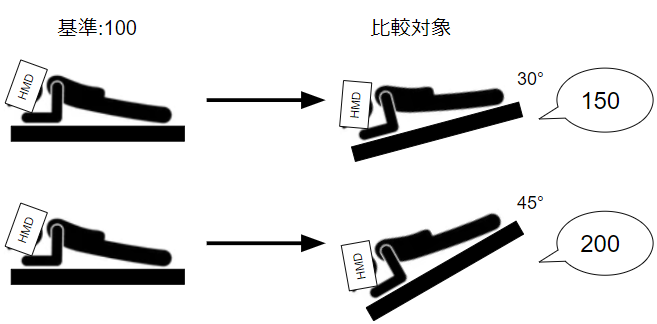
\includegraphics[width=1\linewidth]{fig/マグニチュード法.png}}
  \caption{マグニチュード法例}
  \label{fig:magnitude}

\end{figure}

\section{評価方法}
本実験では落下感覚の比較のためマグニチュード法を用いる。

マグニチュード法は基準となる条件とその比較対象になる条件を連続して実験し,基準に対して測定したい感覚が何倍程度になったかを被験者に回答させる方法であり,これによって感覚などの数値化しづらいものをの数値化を行うことができる.

例えば\figref{fig:magnitude}の場合では基準となる傾きが0度の状態での落下感覚を100として実験し,その後に比較として30度傾けた条件で実験を行っている.そして被験者は基準に対して落下感覚が1.5倍になったと感じたため150と回答している.

その後,同じように基準となる0度の実験の後に,比較対象となる45度を行い被験者は落下感覚が2倍になったと感じたため200と回答している.

\section{検討事項}
本研究の検討事項は3つある.

1つ目は実験の際,落下時に与える視覚,聴覚,姿勢以外の提示情報は何を提示するかという点についてである.
落下感覚にはこれ以外にも風などが関係していることが分かっている\cite{青木誠也2018音と風によって浮遊感を感じさせる装置の制作}.
そのため、視覚,聴覚,姿勢以外に何の要素を加えてどの程度落下感覚を与えて実験を行うか検討する必要がある.

2つ目も同じく実験内容についての検討であり,シミュレーション中に体を傾ける場合,体を傾けるタイミングについてである.
まだこのシミュレーション自体についての検討が足りていないため,体を傾けるタイミングや角度についても検討が必要である.

3つ目は安全性についてである.
本研究で使用するウィンチは人を乗せた物に対しての使用を推奨しておらず,安全機能も最低限のものであるため,怪我人を出さないためにも実験中に起こりうる事故を想定し,それに対しての対策を検討する必要がある.

\section{今後の展望}
まず目指すこととして,体を傾けることのできるデバイスが完成しておらず,実験に着手できないためその作成を第一の目標として作業を進める.

次に,前述したように実験内容を詳細に決定し,安全面についての検討を重ねる.

\section{まとめ}
本研究では,伏臥位の状態のまま角度を変えられるシステムを開発し,それを用いてVR環境で落下する際の伏臥位の角度の違いによって生じる落下感覚の差と,落下中の角度の変化が落下感覚に与える影響について比較と調査を行う.


 \bibliographystyle{junsrt}
\bibliography{ref.bib}   % 参考文献のデータベースファイルを指定する 
\end{document}
